\chapter{Project Methodology}%
\label{method}

\section{Technology}

This project uses two main technologies, which will be outlined here.

The first, is StarCraft II itself. StarCraft II is a real-time strategy game on
the PC\@. % Rest of the description here or in the research section? Probably here.
% An image of SC II is also probably worth adding here.

The bulk of this project is based around the work done by DeepMind, producing
the StarCraft II Learning Environment, which is a Python\cite{python-website}
wrapper for the Blizzard produced API for StarCraft II\cite{bliz-api}. This
environment removes a lot of the traditional issues that come playing
games using machine learning agent. This is because the two main issues, that
is input and unit recognition have been removed, which allows the more interesting
problems to be addressed more easily. This is due to a rich input API that means
passing the result from an agent is much more easy, as well as a large number
of pre-made feature maps, meaning issues such as unit recognition are made much
simpler.

% An image for the SC2LE should either be added here, or in the implementation
% section, to aid the descriptions there. I would think maybe a general one here
% and more specific examples later?

A second reason for using SC2LE was that it is written in Python, which most
of the currently popular machine learning libraries are written in. We chose to
use TensorFlow\cite{abadi2016tensorflow} produced by Google. Primarily,
this was due to its prevalence in the community meaning it had large amounts of
support, as well as documentation. It also allows simple neural networks to be
built up quickly, to help the rapid iterations we will need once we are experimenting
with different network types and parameters. Also, it is easily accelerated on the
GPU, meaning that large speed ups can be gained when running on appropriate hardware.
This hardware is accessible at Leeds University using the ARC machines, which are
part of the High Performance Computing facilities at the University
of Leeds\cite{arc}.

\section{Approach}

The approach taken, and the only one that seemed appropriate for this style of
project, was an iterative agile approach. This allows the iterations to depend
on how the project is progressing, meaning that the focus can be shifted if targets
are reached earlier or later than expected.
When issues or ideas arise, these can be tracked on the GitHub code repository,
which will contain the code for the project, and may also be used for milestones
of progress. This gives a central location for all members to store work, as well
as discuss ideas and bug fixes.

\section{Schedule}

As part of the scoping and planning document, an initial time-scale was made
to plan the time that should be spent on differing parts of the project.
This initial plan can be seen in Figure~\ref{fig:gantt}.

\begin{figure}[h!]
    \centering
    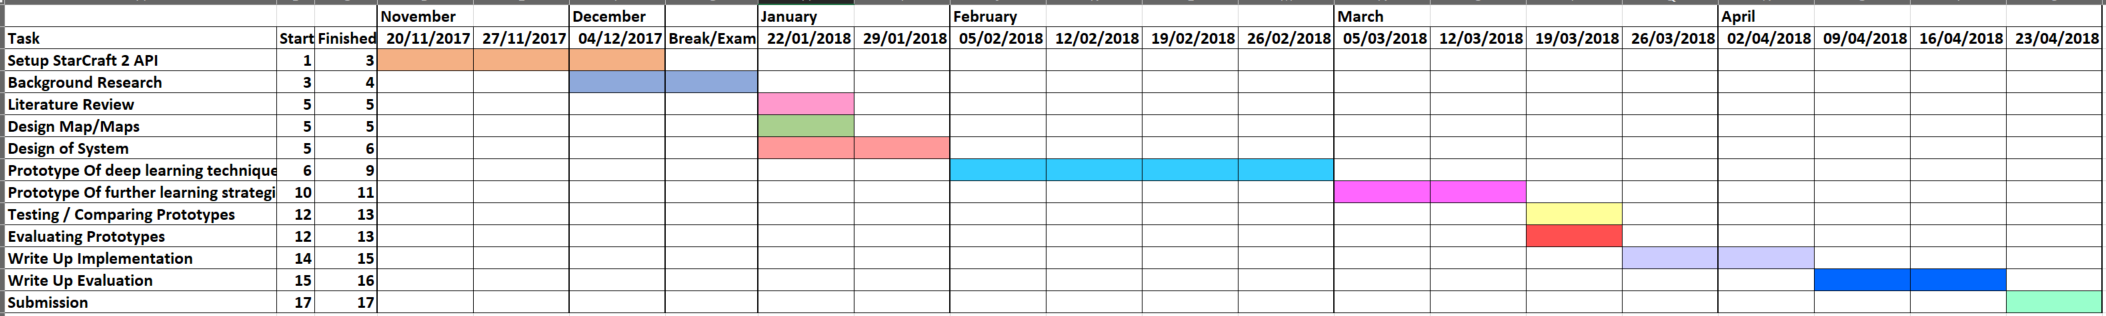
\includegraphics[width=1\textwidth]{gantt}
    \caption{Initial Time Frame}%
    \label{fig:gantt}
\end{figure}

It can be seen that the largest portion of time was given to the prototyping
stage. This was because the definitive scope of that stage is dependant on how
the project progresses, and which styles of learning end up being implemented and
being the most interesting. As such, whilst being a very long part of the project
on the chart, it will actually be made up of lots of small iterations, as described
earlier.

\subsection{Background Research/Literature Review}

In an Exploratory Software project, the research and literature review sections
are some of the most important, both in terms of understanding the problem
space the project is heading in, as well as understanding the styles of
solutions that have been used in both the area and other problems before.
This allows the problem to be fully understood, and to understand the work
and issues that come with various solutions. It can also help inform
the prototypes stage, by giving extra definition in how the prototyping stage
should progress, such as the styles of methods to test and the parameters to tune
in them.

\subsection{Prototypes}

After researching the problem and possible solutions, prototypes of various
solutions need to be produced. These prototypes can vary in both their approach
to the problem as well as being small iterative changes over a previous model
to tune certain parameters. A number of differing prototypes are useful for
various things, mainly to provide more conclusive evaluations later in the report,
since there will be more prototypes to compare against. It is also beneficial to
help identify what features of a prototype are the most useful, since networks
features can be compared and contrasted to see what features consistently give the
best behaviours.

The majority of the project is scheduled in this area, as there is a few
different techniques we can test, as well as further ones that will be found
during the research phase. Spending a lot of time to get a number of differing
agents increases the likelihood of finding what is needed to exhibit intelligent
behaviour and also increases understanding of the project space for further
prototypes.

\subsection{Modifications to Timeline}
% Potentially not needed.
